\section{Results \& Discussion}
\label{sec:Results-Discussion}

\subsection{Scenarios}

The scenarios tested were a combination of the following values for the variables:

\begin{itemize}
    \item \textbf{Operation Policty:} Base, (Intelligent) GPS, CAV
    \item \textbf{Vecicle Arrival Ratio:} 15, 20, 35
    \item \textbf{Traffic Network:} Medium, Large
\end{itemize}

Only the most relevant results are presented.

\subsection{Results}

The experiments yielded fairly consistent results through the scenarios. Most results present are referent to the large network, as the differences between the models are more evident with it. A more comprehensive list of results can be found in Table \ref{tab:table}. As can be observed in Figure \ref{fig:steps-20-large}, the CAV and the Intelligent GPS policies lead to a significantly shorter time until 200 vehicles have arrived at the destination of the large network in comparison to the base case. 
CAV and Intelligent GPS models have obtained quite similar results for Average Travel Time and Average Travel Efficiency, with very similar plots and values at the 200-vehicle mark, as shown by Figures \ref{fig:ate-20-large} and \ref{fig:att-20-large}, with the CAV strategy taking the edge ever so slightly. However, the differences between these two models are made more evident by the Max. Congestion Rate plots, seen in Figure \ref{fig:congestion-20-large}. As presented, the CAV model's correspondent congestion metric slows down growth around the 2.0 value, presenting a much more horizontal plot and achieving much lower and more desirable congestion values overall, whereas the congestion on the other strategies scales near linearly. Even though congestion is not the main metric used to judge the operation policies, it is still an interesting observation. 

\begin{figure}
    \centering
    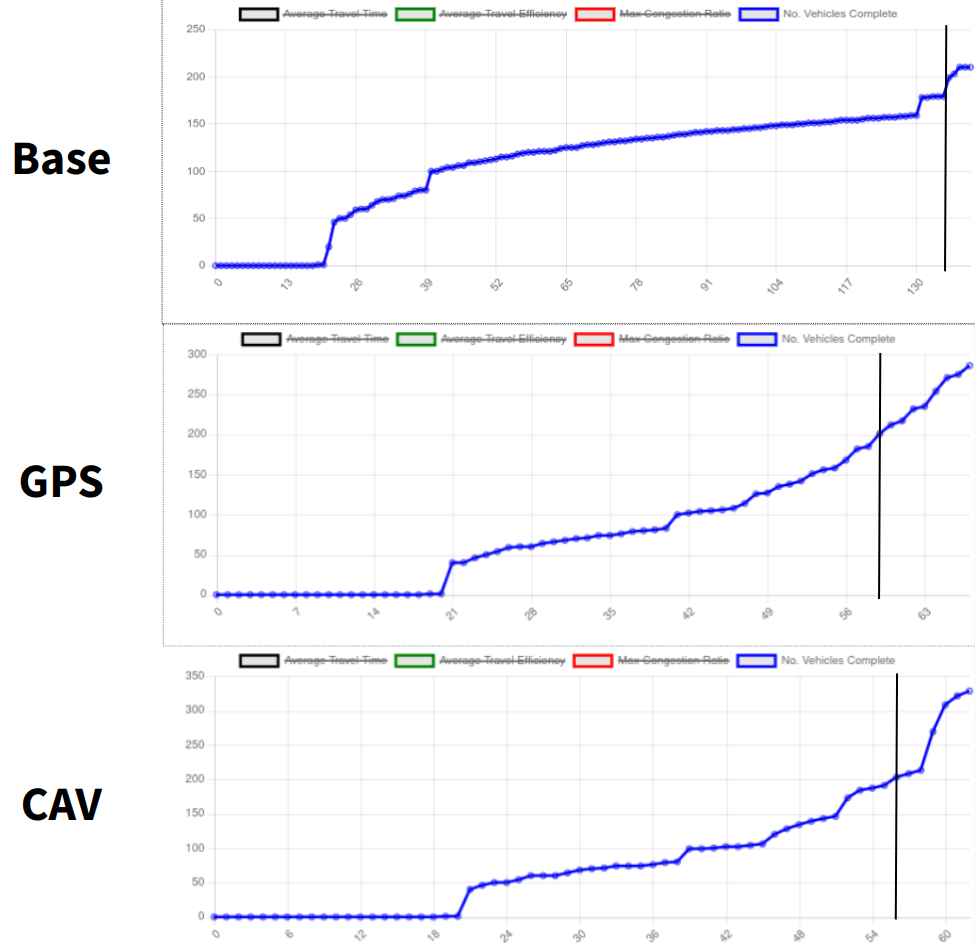
\includegraphics[width=0.45\textwidth]{img/steps-20-large.png}
    \caption{Comparison between the 3 policies on Vehicles Completed per Step for 20 vehicle Arrival Rate in the Large Network}
    \label{fig:steps-20-large}
\end{figure}

\begin{figure}
    \centering
    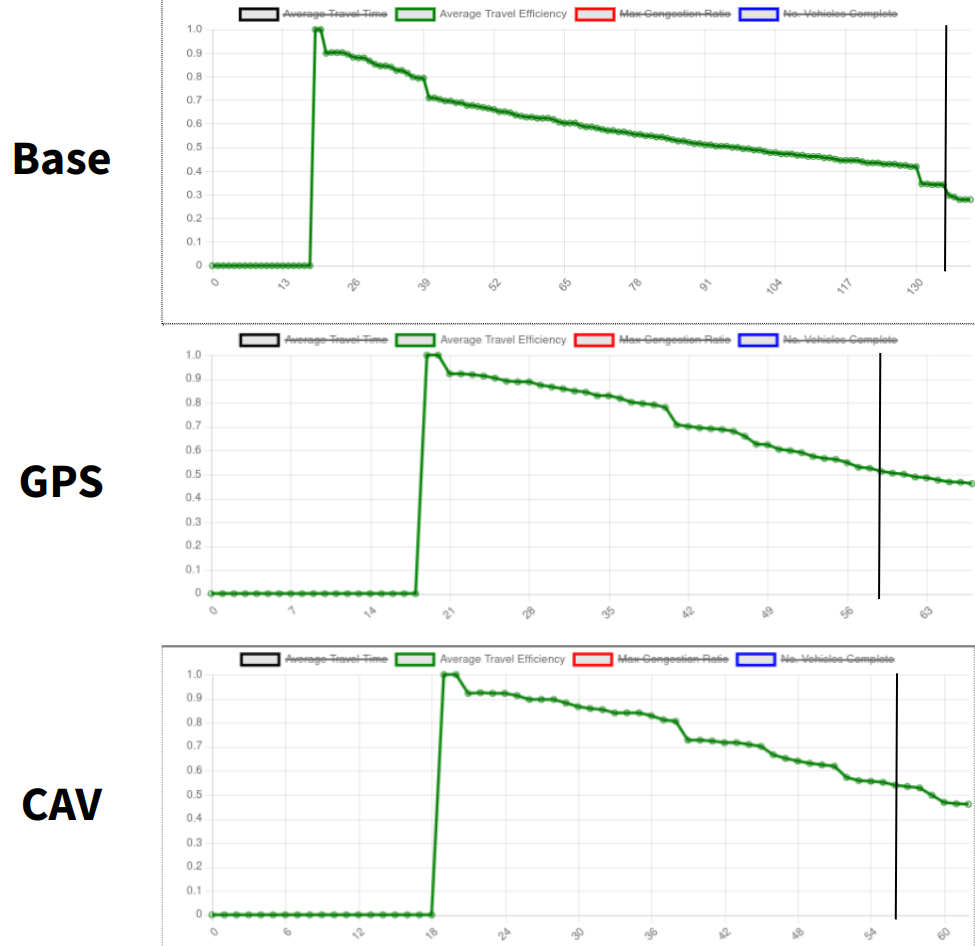
\includegraphics[width=0.45\textwidth]{img/ate-20-large.png}
    \caption{Comparison between the 3 policies on Average Travel Efficiency for 20 vehicle Arrival Rate in the Large Network}
    \label{fig:ate-20-large}
\end{figure}

\begin{figure}
    \centering
    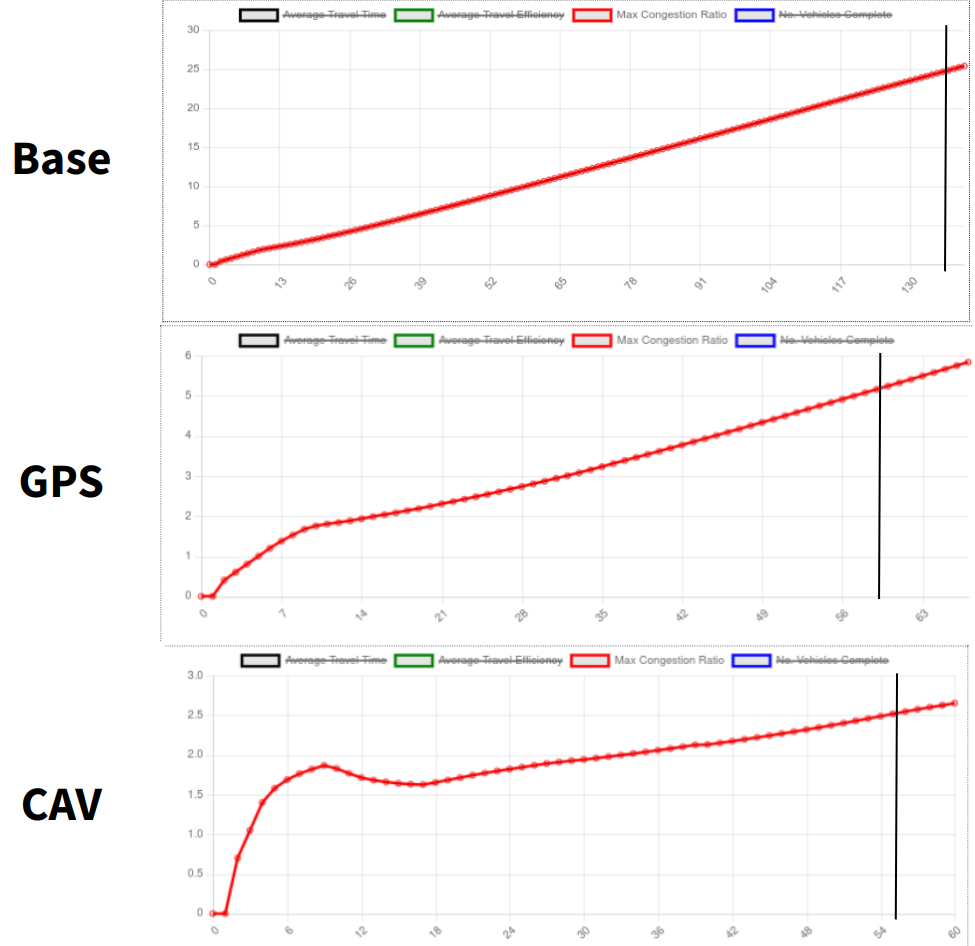
\includegraphics[width=0.45\textwidth]{img/congestion-20-large.png}
    \caption{Comparison between the 3 policies on Average Max. Congestion for 20 vehicle Arrival Rate in the Large Network}
    \label{fig:congestion-20-large}
\end{figure}

\begin{figure}
    \centering
    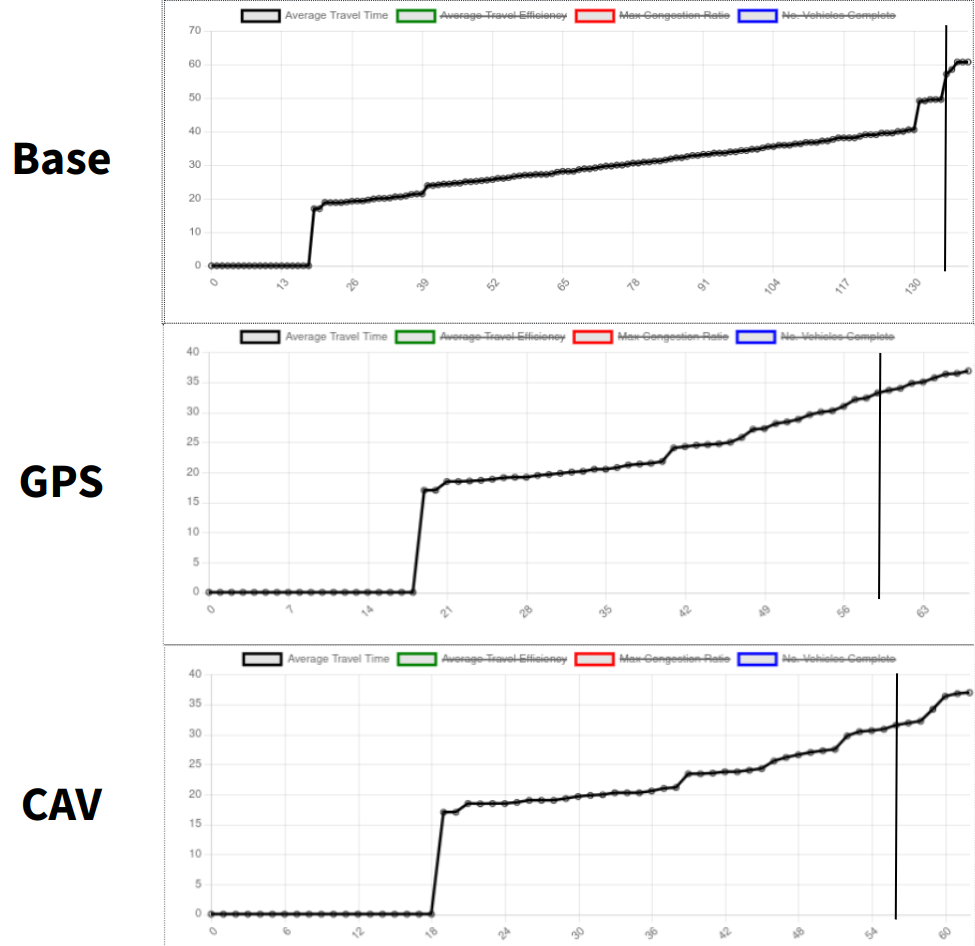
\includegraphics[width=0.45\textwidth]{img/att-20-large.png}
    \caption{Comparison between the 3 policies on Average Travel Time for 20 vehicle Arrival Rate in the Large Network}
    \label{fig:att-20-large}
\end{figure}

\begin{table*}[h]
\centering
\caption{Results by Scenario and Policy}
\begin{tabularx}{\textwidth}{|l|l|X|X|X|X|}
\hline
\textbf{Scenario} & \textbf{Policy} & \textbf{Average Travel Time (s)} & \textbf{Average Max V/C Ratio} & \textbf{Average Travel Efficiency} & \textbf{Vehicles Killed} \\ \hline
\multirow{3}{*}{Medium Model(20)}  & DUMB       & 103.80 & 26.56 & 0.193 & 1226  \\ \cline{2-6} 
                               & HALF\_SMART & 22.32  & 1.16  & 0.896 & 9538  \\ \cline{2-6} 
                               & SMART      & 26.00  & 1.47  & 0.769 & 9218  \\ \hline
\multirow{3}{*}{Large Model(15)}   & DUMB       & 104.45 & 69.86 & 0.163 & 316   \\ \cline{2-6} 
                               & HALF\_SMART & 45.32  & 33.91 & 0.375 & 3728  \\ \cline{2-6} 
                               & SMART      & 44.29  & 1.66  & 0.384 & 6774  \\ \hline
\end{tabularx}
\label{tab:table}
\end{table*}

\subsection{Discussion}

Through the analysis of the results, it can be deduced that:

\begin{itemize}
    \item The base strategy is definitely very far in terms of performance from the other ones, meaning the use of more recent and advanced GPS / path generation apps is justified;
    \item CAVs only present a slight improvement in comparison to the usage of the smart application, most likely due to the fact that the delay imposed is not very impactful in the scenarios examined;
    \item CAVs show significantly lower levels of congestion in comparison to the other options, leading to the conclusion that this strategy originates a more distributed and balanced road network.
\end{itemize}

Both CAV and Intelligent GPS policies fulfilled the performance indicator chosen, meaning both of these techniques are capable of being implemented with success in increasing a traffic network's throughput. However, only the second decision criterion is fulfilled, meaning the enhancement provided by the CAVs in comparison to the strategies already available does not justify its possible costs of implementation. 